\chapter{Project 2: Button}

\section{Overview}
This project adds on to the lessons from the last project. In addition to our LED, we will now also have
a button in our circuit. Over the course of this project, you will:
\begin{itemize}
    \item Create a simple circuit using your breadboard
    \item Write a program that runs in a loop and listens for user input (the button)
    \item Respond to user input by changing the brightness of the LED
\end{itemize}
At the end of this project, your microcontroller should run a MicroPython program which changes the
brightness of the LED when the button is pushed. Let's get started!
\begin{figure}[H]
\centering
    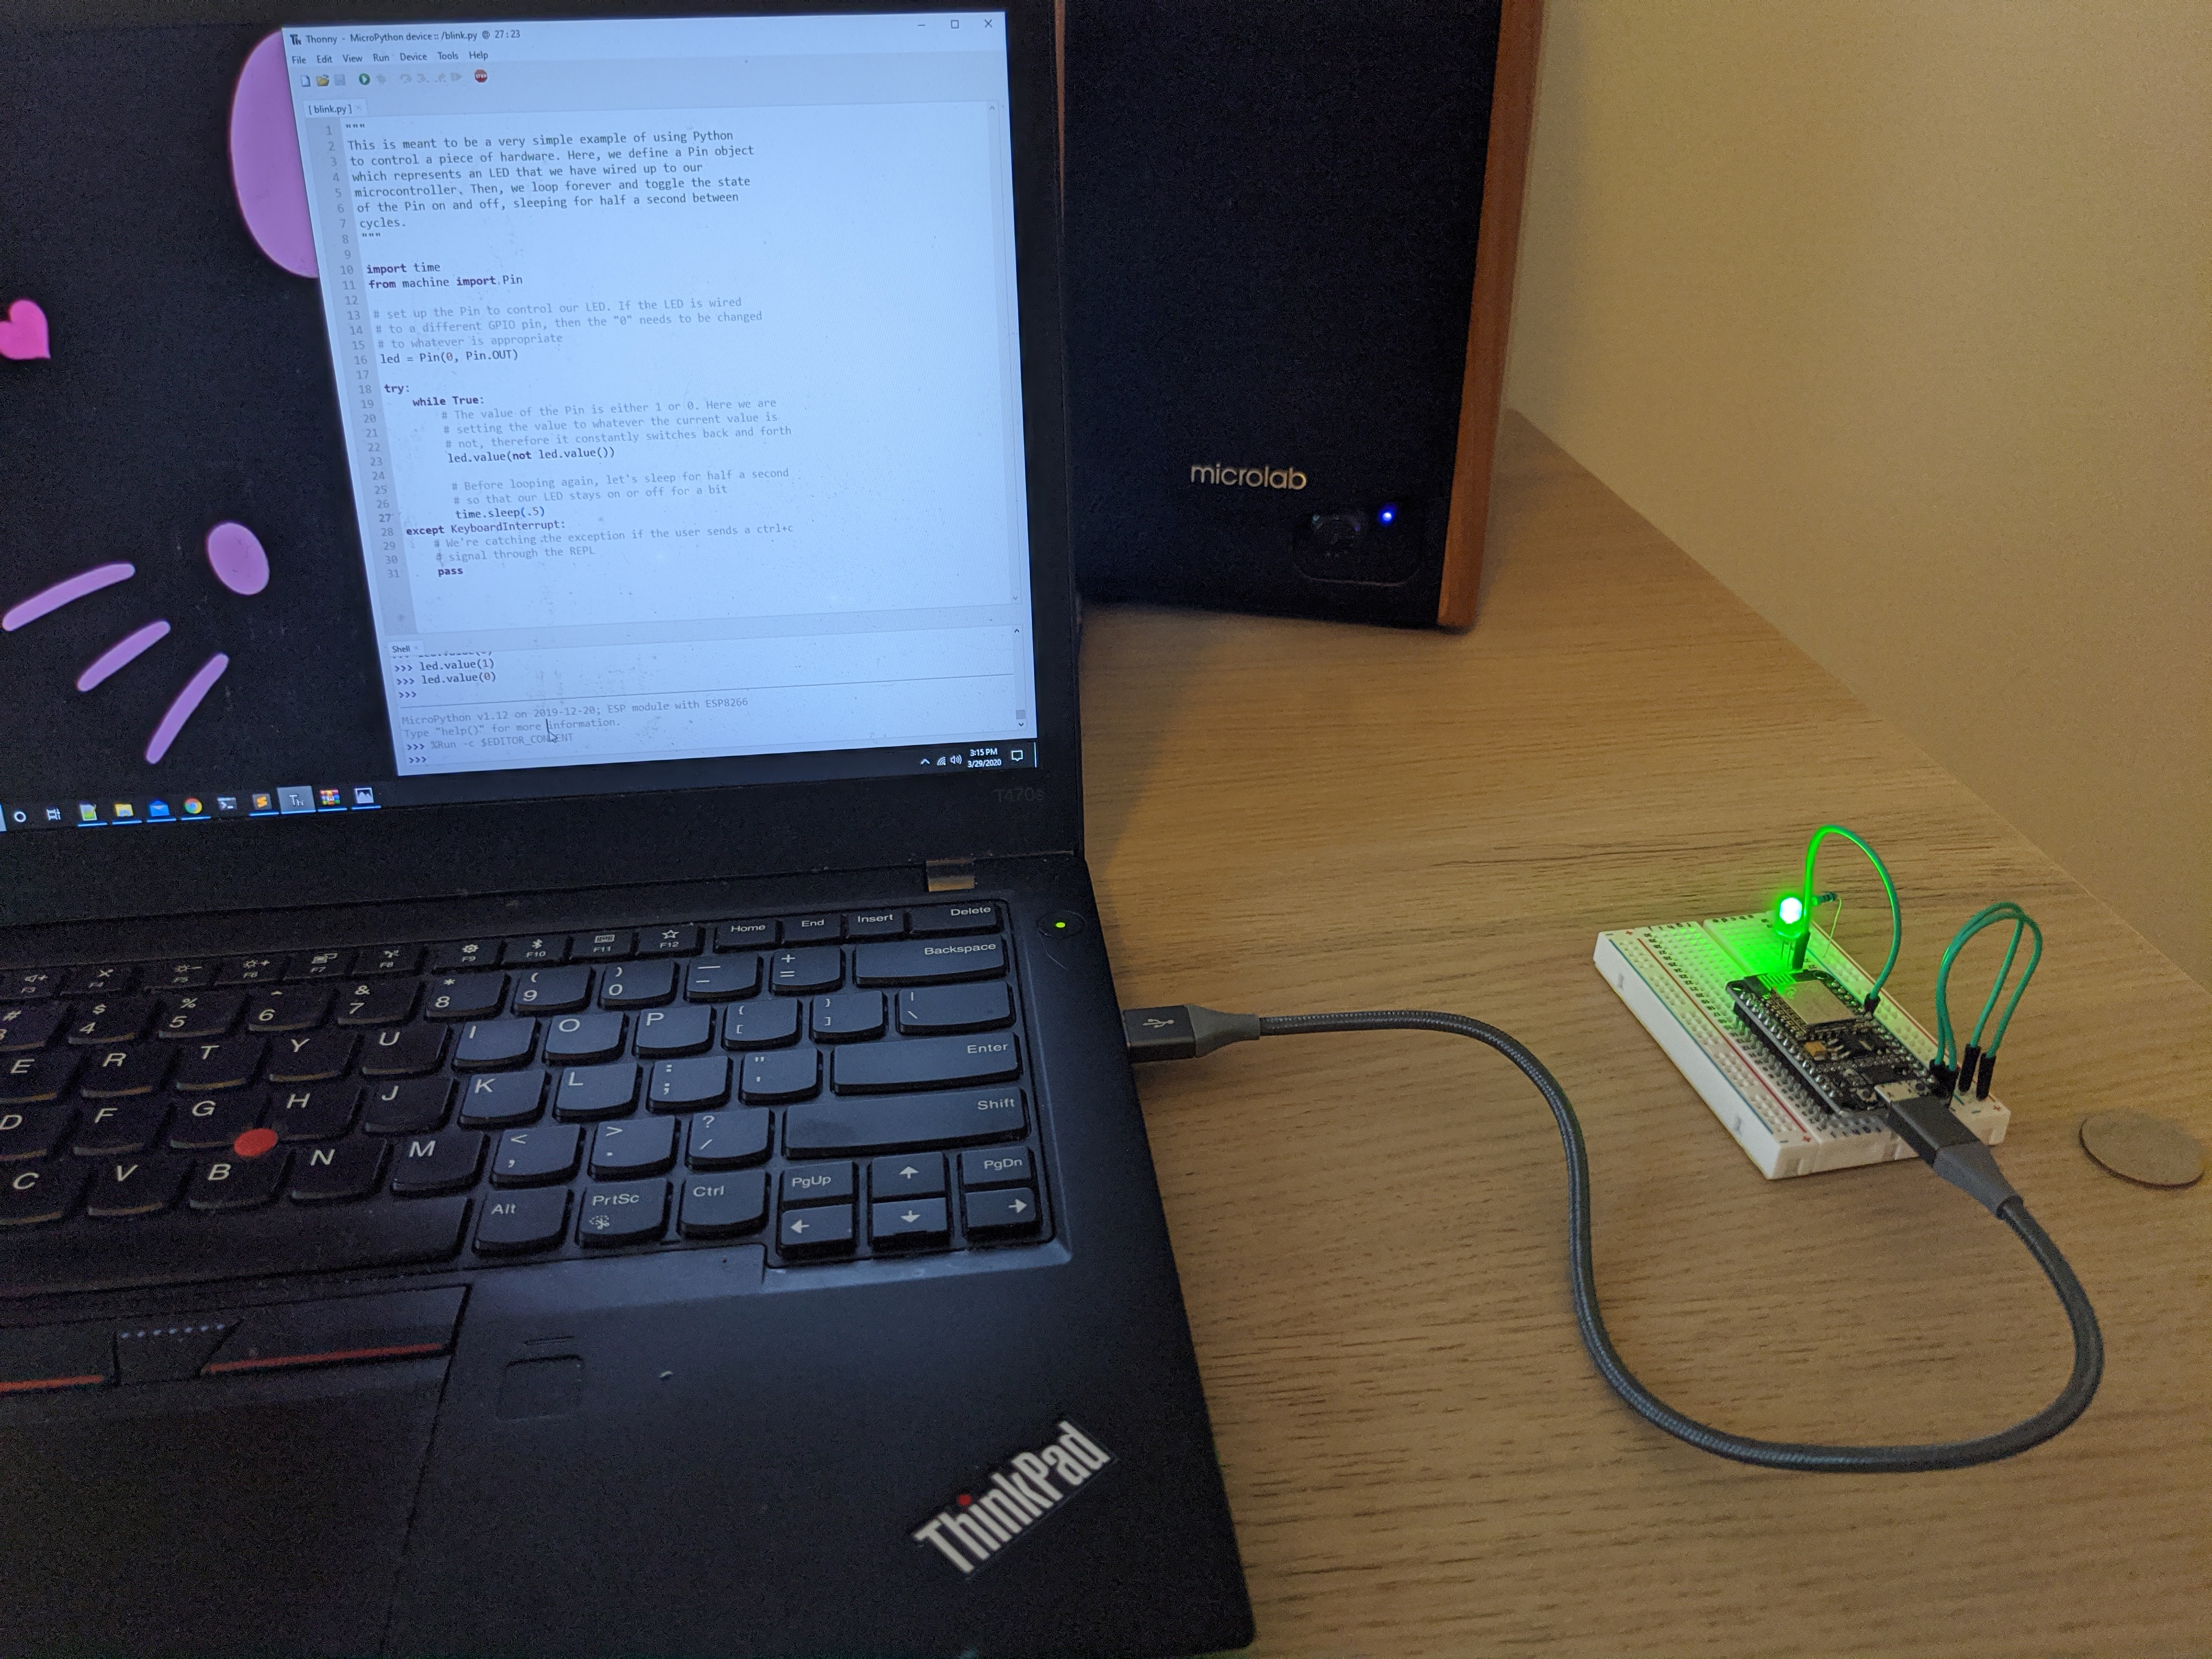
\includegraphics[width=.6\linewidth]{project_2/success!.jpg}
    \caption{The end result should look something like this}
\end{figure}

\pagebreak

\section{Directions}

\subsubsection{Remove previous components}
Before beginning, remove any components from prior chapters including LEDs, buttons, and wires. You may leave the
microcontroller attached to the breadboard.

\subsection{Creating the circuit}
Using jumper cables, you will be assembling a circuit between your microcontroller, your breadboard,
an LED, a pushbutton, and 220\si{\ohm} resistors for the LED and button.

\subsubsection{Attach the microcontroller to the breadboard}
Carefully insert the pins at the bottom of your microcontroller into the breadboard, making sure that the microcontroller is oriented such that:
\begin{itemize}
    \item The pin labeled \textbf{3V3} is inserted in hole at \textbf{Column C, Row 1} of the breadboard (or \textbf{C1}, for short)
    \item The pin labeled \textbf{Vin} is inserted in hole \textbf{J1} of the breadboard
    \item The pin labeled \textbf{D0} is inserted in hole \textbf{C15} of the breadboard
    \item the pin labeled \textbf{A0} is inserted in hole \textbf{J15} of the breadboard
\end{itemize}
You may need to apply more pressure than expected to seat the microcontroller properly in the breadboard. When its over, it should look like this:

\begin{figure}[H]
    \centering
    \includegraphics[width=.6\linewidth]{common/microcontroller_seated_in_breadboard.jpg}
    \caption{So far, so good!}
\end{figure}

\subsubsection{Connect the LED, Button, and Resistors}
\begin{itemize}
    \item Place an LED of your choice (the example image below uses RED) into the breadboard. The longer leg
    should be placed in \textbf{B16} and the shorter leg should be placed in \textbf{B17}.
    \item Place one leg of a resistor (doesn't matter which one) in \textbf{A17} and the other in
    \textbf{A21}.
    \item Place the button so that one connected set of pins (refer to \ref{button_basics} for an
    example) is in \textbf{C28} and \textbf{A28} and the other set is in \textbf{C30} and \textbf{A30}.
    \item Place a resistor between \textbf{E28} and \textbf{C21}. This will provide the low signal that
    the button can switch.
    \item Finally place a resistor between \textbf{E30} and the top negative rail (the blue one).
\end{itemize}

You should be left with something that looks like this:
\begin{figure}[H]
    \centering
    \includegraphics[width=.55\linewidth]{project_2/components_placed.jpg}
    \caption{All of the components except for the jumper wires are now placed.}
\end{figure}

\subsubsection{Connect the necessary jumper wires}
\begin{itemize}
    \item Place one end of a red jumper wire into hole \textbf{J7} of the breadboard and the other end into
    \textbf{E16}. This will provide \textbf{3.3} volts of power to the LED when the program turns it on.
    \item Using a black jumper wire, place one end of the wire into hole \textbf{J2} of the breadboard and the other
    end into \textbf{E21}. This will provide a ground path for the LED through the resistor to complete the circuit.
    \item Place a green jumper wire into hole \textbf{J6} and the other end into \textbf{E30}. This
    will provide the signal to the microcontroller that the button has been pressed.
\end{itemize}

You should be left with something that looks like this:
\begin{figure}[H]
    \centering
    \includegraphics[width=.55\linewidth]{project_2/all_wired_up.jpg}
    \caption{All of the components except for the jumper wires are now placed.}
\end{figure}

\subsection{Programming the microcontroller}

Once all of the wiring is correct, connect the USB cable to the microcontroller and load the IDE to
access it. Refer back to Chapter \ref{ide} for instructions.

Click on the file named "project\_2\_button.py". This will load the code in the editor for this section.
Read through the comments and the code to get a sense for how it works. Once you are ready, you can
click the blue play button in the upper left of the window to start the script.

While the script is running, the LED will toggle between off and 3 different brightness levels. It will
change whenever you press the button.

\section{Review}
In this project, we learned how we can add interactivity to a circuit by using momentary pushbuttons.
These buttons can be read from the microcontroller's code to run a piece of code (called an interrupt)
whenever they are pressed.

\section{Possible Extensions}
If you want to do some experimentation, try these:

\begin{itemize}
    \item Add more brightness levels for the LED to change between
    \item Update the code so that it listens for a secret series of button presses before it will turn the LED on
\end{itemize}
